\documentclass[letterpaper]{article}
\usepackage[utf8]{inputenc}
\usepackage{amsmath}
\usepackage[margin=3cm]{geometry}
\usepackage{tikz}


\begin{document}

\title{{\bf Ejercicios}} 
\author{Analítica de Datos  \\
	Pontificia Universidad Javeriana}

\date{}

\maketitle

\section{Intervalos de Confianza}

\subsection{Ejercicio Resuelto}
\begin{itemize}
	\item Se quiere conocer la permanencia media de los pacientes de un hospital, con el fin de estudiar una posible ampliación del mismo. Se tienen datos referidos a la estancias, expresada en días, de 800 pacientes, obteniéndose los siguientes resultados: $\bar{X}$ = 8,1 días; $s$ = 9 días. Se
	pide obtener un intervalo de confianza del 95\% para la estancia media
	
	
	\item {\bf Solución:} Lo primero es calcular el nivel de significancia (error esperado) dado el nivel de confianza que presenta el enunciado. El nivel de significancia se denota con la letra $\alpha$. Por lo tanto:
	
	$$\alpha=100\% - nivel \, de\, confianza$$
	$$\alpha=100\%-95\%=5\%$$
	
	Dado este error esperado, ahora se debe encontrar el valor \emph{Z critico}, simbolizado $Z_{\alpha}$. En este caso tenemos que encontrar el $Z_{\alpha}$ para un nivel de significancia igual al 5\%. Por lo tanto, buscamos en la tabla de la normal el valor $Z$ para el cual 97.5\% de las observaciones caigan debajo de ese valor. ¿Por qué el 97.5\%? Al observar la distribución de abajo, se observa que ambas áreas rojas deben sumar 5\%, por lo tanto, cada una debe sumar la mitad. Si el área roja de la derecha es igual al 2.5\% del área total, el resto es igual a $100-2.5=97.5\%$. Al buscar este valor en la tabla de la distribución normal, se encuentra que el valor Z es igual a $1.96$. Considerando la simetría de la curva normal, se sabe que el valor que divide el $2.5\%$ del área roja de la izquierda con respecto al área verde es $-1.96$.
	
	\begin{center}
		
		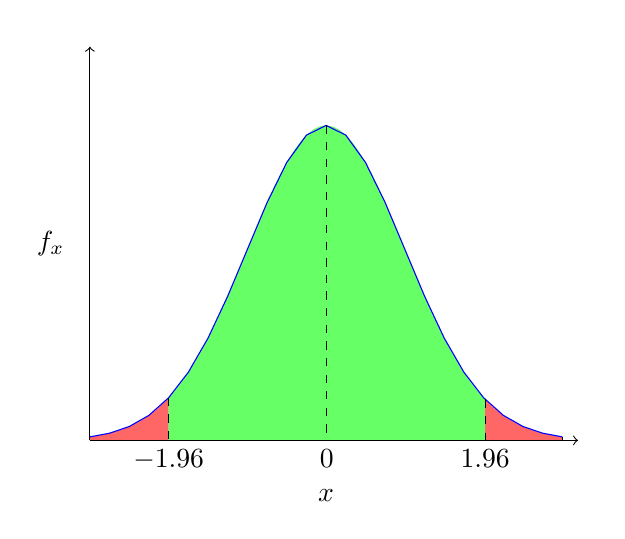
\begin{tikzpicture}
		% define normal distribution function 'normaltwo'
		\def\normaltwo{\x,{4*1/exp(((\x-3)^2)/2)}}
		
		% input y parameter
		\def\x{0}
		\def\y{1}
		\def\w{5.02}
		\def\q{6}
		\def\z{3.01}
		
		
		% this line calculates f(y)
		\def\fx{4*1/exp(((\x-3)^2)/2)}
		\def\fy{4*1/exp(((\y-3)^2)/2)}
		\def\fz{4*1/exp(((\z-3)^2)/2)}
		\def\fw{4*1/exp(((\w-3)^2)/2)}
		\def\fq{4*1/exp(((\q-3)^2)/2)}
		% Shade orange area underneath curve.
		\fill [fill=red!60] (\x,0) -- plot[domain=\x:\y] (\normaltwo) -- ({\y},0) -- cycle;
		\fill [fill=green!60] (\y,0) -- plot[domain=\y:\z] (\normaltwo) -- ({\z},0) -- cycle;
		\fill [fill=green!60] (\z,0) -- plot[domain=\z:\w] (\normaltwo) -- ({\w},0) -- cycle;
		\fill [fill=red!60] (\w,0) -- plot[domain=\w:\q] (\normaltwo) -- ({\q},0) -- cycle;
		% Draw and label normal distribution function
		\draw[color=blue,domain=0:6] plot (\normaltwo) node[right] {};
		
		% Add dashed line dropping down from normal.
		\draw[dashed] ({\x},{\fx}) -- ({\x},0) node[below] {};
		\draw[dashed] ({\y},{\fy}) -- ({\y},0) node[below] {$-1.96$};
		\draw[dashed] ({\z},{\fz}) -- ({\z},0) node[below] {$0$};
		\draw[dashed] ({\w},{\fw}) -- ({\w},0) node[below] {$1.96$};
		\draw[dashed] ({\q},{\fq}) -- ({\q},0) node[below] {};
		% Optional: Add axis labels
		\draw (-.2,2.5) node[left] {$f_x$};
		\draw (3,-.5) node[below] {$x$};
		
		% Optional: Add axes
		\draw[->] (0,0) -- (6.2,0) node[right] {};
		\draw[->] (0,0) -- (0,5) node[above] {};
		
		\end{tikzpicture}
	\end{center}
	Encontrado el valor \emph{Z crítico}, se calcula el error estándar para la distribución de medias muestrales. En este caso:
	$$s_{\bar{X}}=\dfrac{s_X}{\sqrt{n}}=\dfrac{9}{\sqrt{800}}=0,318$$
	Una vez calculado el error estándar, este se multiplica por $Z_{\alpha}$ para obtener el término o margen del error:
	$$Margen\, de\, error=Z_{\alpha}*s_{\bar{X}}=1,96*0,318=0,62$$
	El intervalo de confianza de una media poblacional es una media muestral más y menos un término de error, la fórmula general para calcular el intervalo de confianza es la siguiete:
	
	$$IC\, Superior=\bar{X}+Z_{\alpha}*s_{\bar{X}}=8,1+0,62=8,72$$
	$$IC\, Inferior=\bar{X}-Z_{\alpha}*s_{\bar{X}}=8,1-0,62=7,48$$
	Estoy 95\% seguro que la estancia media de los pacientes está entre 7,4 y 8,72 días.
\end{itemize}

\subsection{Ejercicios}
\begin{enumerate}
	\item Una muestra aleatoria simple de 25 estudiantes responde a un test de inteligencia, obteniendo una media de 100 puntos. Se sabe por experiencia que la variable “inteligencia de todos los estudiantes” es normal con una desviación estándar igual a 10, pero se desconoce la media. ¿Entre qué límites se hallará la verdadera inteligencia media de todos los estudiantes,
	con un nivel de confianza de 99\%? {\bf Rta: ICS=105,1 ICI=94,9}
	\item  Se asume que la recaudación diaria de las tiendas de un barrio determinado es una variable aleatoria que se aproxima a una distribución normal con una desviación estándar de 328000 pesos. Se ha extraído una muestra de 100 tiendas de dicho barrio, obteniéndose que la recaudación diaria media asciende a 1'248.000 pesos. Calcular:
	\begin{enumerate}
		\item El intervalo de confianza para la recaudación media con un nivel de confianza del 99\%. {\bf Rta: ICS=1'331.640 ICI=1'164.360}
		\item El tamaño muestral mínimo necesario para conseguir, con un nivel de confianza del 95\%, un error en la estimación de la recaudación diaria media menor de 127.000 pesos. {\bf Rta: $n > 26$}
	\end{enumerate}
	\item En una encuesta se pregunta a 10.000 personas cuántos libros lee al año, obteniéndose una media de 5 libros. Se sabe que la población tiene una distribución normal con desviación estándar de 2. Hallar un intervalo de confianza al 80\% para la media poblacional. {\bf Rta: ICS=5,0256 ICI=4,9744}
	\item Se quiere estimar el sueldo medio de un trabajador de transporte público. Se toma para ello una muestra de 625 de estos trabajadores y se obtiene un sueldo medio muestral de 1'480.000 pesos. Si la desviación estándar es igual a 250.000 pesos:
	\begin{enumerate}
		\item Con un nivel de confianza del 90\%, determine el intervalo de confianza para el sueldo medio de un trabajador del transporte público. {\bf Rta: ICS=1'496.500 ICI=1'463.500}
		\item Si se quiere que el error máximo de la estimación sea de 10.000 pesos, hallar el tamaño de la muestra que se debe tomar considerando un nivel de confianza del 99\%. {\bf Rta: $n > 4065$}
		
	\end{enumerate}
	\item Para hacer un estudio sobre el precio/día de una habitación doble en hoteles de cuatro estrellas en Cartagena, se elige una muestra de 64 de estos hoteles y se obtiene un precio/día medio de 56 mil pesos con una desviación típica de 6 mil pesos. Determine el intervalo de confianza para el precio/día medio de una habitación doble en un
	hotel de cuatro estrellas en Cartagena con un nivel de confianza del 97\%. {\bf Rta: ICS=57,62 ICI=54,38}
	\item Se ha obtenido una muestra al azar de 150 vendedores de una Editorial para estimar la proporción de vendedores en la Editorial que no alcanza un límite de ventas mínimo establecido por la dirección.
	De entre los seleccionados, 50 no han conseguido llegar al límite de ventas mínimo establecido.
	\begin{enumerate}
		\item Calcule el intervalo de confianza para la proporción de trabajadores en la Editorial que no alcanza el límite al 80\%. {\bf Rta: ICS=0,38 ICI=0,28}
		\item Calcule el intervalo de confianza para la proporción de trabajadores en la Editorial que no alcanza el límite al 99\%. {\bf Rta: ICS=0,43 ICI=0,23}
	\end{enumerate}
\end{enumerate}

\end{document}